\documentclass[10pt,letterpaper,english]{beamer}

\usepackage{ragged2e}
\justifying

\usetheme{default}
\setbeamertemplate{navigation symbols}{\textcolor{blue}{\insertframenumber ~/ \inserttotalframenumber}}

\usepackage{xstring}
\usepackage{pgfpages}
\makeatletter
\IfSubStr{\@classoptionslist}{handout}
  {\pgfpagesuselayout{2 on 1}[letterpaper,border shrink=5mm]}
  {}
\makeatother

\usepackage{amsmath,amssymb,amsthm}
\usepackage{stmaryrd}
\usepackage{enumerate}
\usepackage{stfloats}
\usepackage{bbm}
\usepackage{pdfpages}
\usepackage{framed}
\usepackage{tabularx}
\usepackage[normalem]{ulem}
\usepackage{ifthen}

\usepackage{tikz,pgf,pgfplots}
\usepackage{algorithm,algorithmic}
\usepgflibrary{shapes}
\usetikzlibrary{%
  arrows,%
  arrows.meta,
  shapes.misc,% wg. rounded rectangle
  shapes.arrows,%
  shapes,%
  calc,%
  chains,%
  matrix,%
  positioning,% wg. " of "
  scopes,%
  decorations.pathmorphing,% /pgf/decoration/random steps | erste Graphik
  shadows,%
  backgrounds,%
  fit,%
  petri,%
  quotes
}

%\pgfplotsset{compat=1.12}

%\usetheme{Frankfurt}
%\usecolortheme{ldpc}
\useinnertheme{rounded}
\usecolortheme{whale}
\usecolortheme{orchid}


\newcommand{\ul}[1]{\underline{#1}}
\renewcommand{\Pr}{\mathbb{P}}

\newcommand{\getpdfpages}[2]{\begingroup
  \setbeamercolor{background canvas}{bg=}
  \addtocounter{framenumber}{1}
  \includepdf[pages={#1},%
  pagecommand={%
    \expandafter\def\expandafter\insertshorttitle\expandafter{%
      \insertshorttitle\hfill\insertframenumber\,/\,\inserttotalframenumber}}%
  ]{#2}
  \endgroup}

\newcommand{\backupbegin}{
   \newcounter{finalframe}
   \setcounter{finalframe}{\value{framenumber}}
}
\newcommand{\backupend}{
   \setcounter{framenumber}{\value{finalframe}}
}

 \setbeamercolor{bibliography entry author}{fg=black}
 \setbeamercolor{bibliography entry title}{fg=black}
 \setbeamercolor{bibliography entry location}{fg=black}
 \setbeamercolor{bibliography entry note}{fg=black}
 
 \setbeamerfont{bibliography item}{size=\footnotesize}
 \setbeamerfont{bibliography entry author}{size=\footnotesize}
 \setbeamerfont{bibliography entry title}{size=\footnotesize}
 \setbeamerfont{bibliography entry location}{size=\footnotesize}
 \setbeamerfont{bibliography entry note}{size=\footnotesize}
 \setbeamertemplate{bibliography item}{\insertbiblabel}
 
\newlength\tikzwidth
\newlength\tikzheight

\def\checkmark{\tikz\fill[scale=0.4](0,.35) -- (.25,0) -- (1,.7) -- (.25,.15) -- cycle;}
\def\greencheck{{\color{green}\checkmark}}
\def\scalecheck{\resizebox{\widthof{\checkmark}*\ratio{\widthof{x}}{\widthof{\normalsize x}}}{!}{\checkmark}}
\def\xmark{\tikz [x=1.4ex,y=1.4ex,line width=.2ex, red] \draw (0,0) -- (1,1) (0,1) -- (1,0);}
\def\redx{{\color{red}\xmark}}

\renewcommand{\footnotesep}{-2pt}

\newif\ifslow
\slowtrue

\newcommand{\mc}[1]{\mathcal{#1}}
\newcommand{\mbb}[1]{\mathbb{#1}}
%\newcommand{\expt}{\mbb{E}}
%\newcommand{\dd}{\mathrm{d}}
\newcommand{\Interior}[1]{\ensuremath{{#1}^{\circ}}}
\newcommand{\Closure}[1]{\ensuremath{\overline{#1}}}
\newcommand{\Complement}[1]{\ensuremath{{#1}^{c}}}

\newcommand{\Expect}{\ensuremath{\mathrm{E}}}
\newcommand{\vecnot}{\underline}
\newcommand{\RealNumbers}{\ensuremath{\mathbb{R}}}
\newcommand{\RationalNumbers}{\mathbb{Q}}
\newcommand{\ComplexNumbers}{\mathbb{C}}
\newcommand{\Real}{\mathrm{Re}}
\newcommand{\Span}{\mathrm{span}}
\newcommand{\Rank}{\mathrm{rank}}
\newcommand{\Nullity}{\mathrm{nullity}}
\newcommand{\Trace}{\mathrm{tr}}
\newcommand{\Diag}{\mathrm{diag}}
\newcommand{\dd}{\mathrm{d}}
\DeclareMathOperator*{\esssup}{ess\,sup}

% Use < , > inner product
\newcommand{\inner}[2]{{\left\langle #1 \mskip2mu , #2 \right\rangle}}
\newcommand{\tinner}[2]{{\langle #1 \mskip1mu , #2 \rangle}}

% Use < | > inner product
%\newcommand{\inner}[2]{{\left\langle #1 \mskip2mu \middle| \mskip2mu #2 \right\rangle}}
%\newcommand{\tinner}[2]{{\langle #1 \mskip1mu | \mskip1mu  #2 \rangle}}




\begin{document}

\ifslow

\title{ECE 586: Vector Space Methods \\ Alternating Projection and Optimization}
\author{Henry D. Pfister \\ Duke University}
\date{November 18th--25th, 2019}
\maketitle


\begin{frame}{5.3: Convexity}

\vspace{-1mm}

\begin{minipage}{0.75\textwidth}
Convexity is a nice property of sets, spaces, and functionals that simplifies analysis and optimization.

\begin{definition}[convex set]
Let $V$ be a vector space over $\RealNumbers$.
The subset $A \subseteq V$ is called a \textcolor{blue}{convex set} if, for all $\vecnot{a}_1,\vecnot{a}_2 \in A$ and $\lambda\in(0,1)$, we have $\lambda \vecnot{a}_1 + (1-\lambda) \vecnot{a}_2 \in A$.
It is \textcolor{blue}{strictly convex} if, for all $\vecnot{a}_1,\vecnot{a}_2 \in \Closure{A}$ and $\lambda\in(0,1)$,
%we have
$\lambda \vecnot{a}_1 + (1-\lambda) \vecnot{a}_2 \in \Interior{A}$.
\end{definition}
\end{minipage}
\hfill
\begin{minipage}{0.22\textwidth}
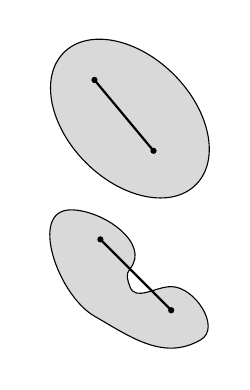
\begin{tikzpicture}[rotate=270,scale=0.75]
    \draw[rotate=-45,fill=gray!30] (-1.8,-1.8) ellipse (30pt and 45pt);
    \draw[thick] (-3.2,-0.6) -- (-2.0,0.4);
    \fill (-3.2,-0.6) circle[radius=1.5pt];
    \fill (-2.0,0.4) circle[radius=1.5pt];
    
    \draw[fill=gray!30] (0,0) to [out=140,in=90] (-1,-1)
    to [out=-90,in=240] (0.8,-0.6)
    to [out=60,in=-60] (1.2,1.2)
    to [out=120,in=90] (0.3,0.7)
    to [out=-90,in=20] (0.3,0)
    to [out=200,in=-40] (0,0);
    \draw[thick] (-0.5,-0.5) -- (0.7,0.7);
    \fill (-0.5,-0.5) circle[radius=1.5pt];
    \fill (0.7,0.7) circle[radius=1.5pt];
\end{tikzpicture}
\end{minipage}

\begin{definition}[convex function]<2->
\begin{minipage}{0.70\textwidth}
Let $V$ be a vector space, $A \subseteq V$ be a convex set, and $f \colon V \rightarrow \RealNumbers$ be a functional.
The functional $f$ is called \textcolor{blue}{convex} on $A$ if, for all $\vecnot{a}_1,\vecnot{a}_2 \in A$ and $\lambda\in(0,1)$, \vspace{-1mm}
\[ f( \lambda \vecnot{a}_1 + (1-\lambda) \vecnot{a}_2 ) \leq \lambda f( \vecnot{a}_1 ) + (1-\lambda) f ( \vecnot{a}_2 ). \vspace{-1mm} \]
It is \textcolor{blue}{strictly convex} if equality implies $\vecnot{a}_1 = \vecnot{a}_2$.
\end{minipage}\hspace{-3mm}
\begin{minipage}{0.29\textwidth}
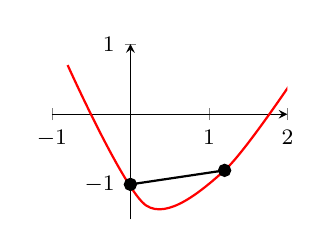
\begin{tikzpicture}
  \begin{axis}[axis x line=center,
    axis y line=center, small,width=1.8in,height=1.5in,xmin=-1,xmax=2,ymin=-1.5,ymax=1]
     \addplot[mark=*, thick, black] coordinates {(0,-1)(1.2,-0.8)};
     \addplot[red,smooth,thick,-] coordinates  {
    (-0.8,0.7) (0.2,-1.3) (1.2,-0.8) (2.2,0.7)};
  \end{axis}
\end{tikzpicture}
\end{minipage}
\end{definition}

\end{frame}

\begin{frame}{5.3: Convex Optimization}

\begin{definition}
Let $(X,\|\cdot\|)$ be a normed vector space.
Then, a real functional $f \colon X \rightarrow \RealNumbers$ achieves a \textcolor{blue}{local minimum value} at $\vecnot{x}_0 \in X$ if: \\ \hspace{3mm}  there is an $\epsilon > 0$ such that, for all $\vecnot{x}\in X$ satisfying $\| \vecnot{x} - \vecnot{x}_0 \| < \epsilon$, we have  $f(\vecnot{x}) \geq f(\vecnot{x}_0)$.
If the bound holds for all $x\in X$, then the local minimum is also a \textcolor{blue}{global minimum value}.
\end{definition}

\vspace{2mm}

\begin{theorem}<2->
Let $(X,\|\cdot\|)$ be a normed vector space, $A \subseteq X$ be a convex set, and $f \colon X \rightarrow \RealNumbers$ be a convex functional on $A$.
Then, \textcolor{blue}{any local minimum value of $f$ on $A$ is a global minimum value on $A$}.
If the functional is strictly convex on $A$ and achieves a local minimum value on $A$, then there is a unique point $\vecnot{x}_0 \in A$ that achieves the global minimum value on $A$.
\end{theorem}

\vspace{1mm}

\visible<2->{Prove theorem on whiteboard and discuss convexity of induced norm}

\end{frame}

\begin{frame}{5.3: Convex Optimization and Derivatives}

\begin{minipage}{0.55\textwidth}
Let $(X,\|\cdot\|)$ be a normed vector space and $f \colon X \rightarrow \RealNumbers$ be a convex functional on a convex set $A \subseteq X$.
\end{minipage}
\begin{minipage}{0.44\textwidth}\hspace{3mm}
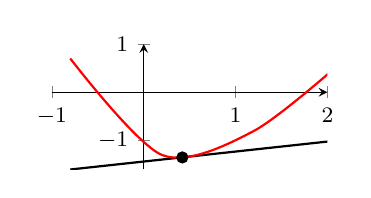
\begin{tikzpicture}
  \begin{axis}[axis x line=center,
    axis y line=center, small,width=2in,height=1.25in,xmin=-1,xmax=2,ymin=-1.6,ymax=1]
     \addplot[mark=none, thick, black] coordinates {(-0.8,-1.6)(2.2,-0.98)};
     \addplot[red,smooth,thick,-] coordinates  {
    (-0.8,0.7) (0.2,-1.3) (1.2,-0.8) (2.2,0.7)};
    \addplot[mark=*] coordinates {(0.42,-1.35)};
  \end{axis}
\end{tikzpicture}
\end{minipage}

\begin{theorem}
If $f$ has a directional derivative  at $\vecnot{x}_0 \in A$ in the direction $\vecnot{x}-\vecnot{x}_0$, then \vspace{-1mm}
\[ f(\vecnot{x}) \geq f(\vecnot{x}_0) + f'(\vecnot{x}_0)(\vecnot{x}-\vecnot{x}_0) \vspace{-1mm} \]
for all $\vecnot{x}\in A$.
If $f$ is strictly convex then the inequality is strict for $\vecnot{x}\neq \vecnot{x}_0$.
\end{theorem}

\vspace{1mm}

\begin{corollary}<2->
If $f$ has directional derivatives in all directions at $\vecnot{x}_0 \in A$ and they all equal zero, then \vspace{-2mm}
\[ f(\vecnot{x}_0) = \min_{\vecnot{x}\in A} f(\vecnot{x}). \vspace{-2mm} \]
If $f$ is strictly convex, then $\vecnot{x}_0$ is the unique minimizer over $A$.
\end{corollary}

\visible<2->{Prove corollary on whiteboard}

\end{frame}


\begin{frame}{4.6: Projection onto Convex Sets}

\begin{minipage}{0.44\textwidth}
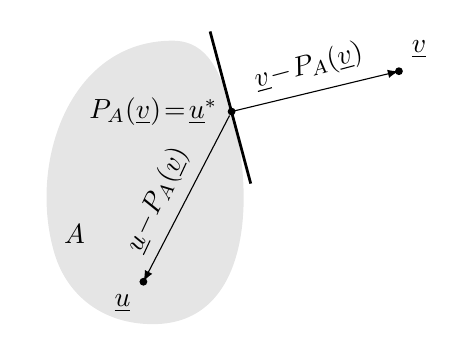
\begin{tikzpicture}[yscale=0.9,bullet/.style={circle,fill,inner sep=1.00pt,node contents={}}]
 \draw[-latex] (0,0) node[bullet,label=left:{$P_A(\vecnot{v}) \!=\! \vecnot{u}^*$},alias=PC]  -- (15:2.2) node[midway,sloped,above=0.25mm] {$\vecnot{v}\!-\! P_A(\vecnot{v})$}
    node[bullet,label=above right:$\vecnot{v}$,alias=v];
\draw[-latex] (PC) -- ++ (-115:2.65) node[pos=0.57,above=0.25mm,sloped]{$\vecnot{u}\!-\! P_A(\vecnot{v})$}     node[bullet,label=below left:$\vecnot{u}$];
\fill[black,fill,opacity=0.1] (PC) to[out=105,in=0] ++ (-0.75,1) to[out=180,in=105] ++ (-1.5,-3)
 node[above right,opacity=1]{$A$} to[out=-75,in=180] ++ (1.25,-1) to[out=0,in=-75] node[sloped, inner xsep=10mm, inner ysep=0, opacity=1, fill=black, pos=0.999] {} cycle;
\end{tikzpicture}
\end{minipage}
\begin{minipage}{0.55\textwidth}
\hspace{3mm} The projection of vectors onto subspaces can be generalized to convex sets\\[-2mm]

For Hilbert space $V$ and closed convex set $A\subseteq V$, let $P_{A}:V\rightarrow A$ denote the orthogonal projection of $\vecnot{v}\in V$ onto $A$: \vspace{-1mm}
\[
P_A (\vecnot{v}) \triangleq \arg \min_{\vecnot u\in A}\left\Vert \vecnot u-\vecnot v\right\Vert \vspace{-1mm} 
\]
\end{minipage}

\begin{theorem}<1->
The orthogonal projection of $\vecnot v\in V$ onto a closed convex set $A\subseteq V$ exists and is unique.
\end{theorem}

\begin{theorem}<2->
For any $\vecnot{v} \notin A$, a necessary and sufficient condition for $\vecnot{u}^* = P_A (\vecnot{v})$ is that $\langle \vecnot{v}-\vecnot{u}^* \,|\, \vecnot{u}-\vecnot{u}^* \rangle \leq 0$ for all $\vecnot{u}\in A$.
\end{theorem}

\visible<3->{Prove theorem on whiteboard for compact $A$ via convex optimization}
\end{frame}


\begin{frame}{Alternating Projection for Subspaces}

Suppose $P_{U}$ and $P_{W}$ are orthogonal projections onto closed subspaces $U$ and $W$ of a Hilbert space $V$. For an arbitrary $\vecnot v_{0}\in V$, what is the behavior of the alternating projection 
\begin{equation*}
\vecnot v_{n+1}=\begin{cases}
P_{U}\vecnot v_{n} & \text{if }n\text{ is even}\\
P_{W}\vecnot v_{n} & \text{if }n\text{ is odd}.
\end{cases}
\end{equation*}
Since $P_{U}\vecnot v=\vecnot v$ (resp. $P_{W}\vecnot v=\vecnot v$) if and only if $\vecnot v\in U$ (resp. $\vecnot v\in W$), it is easy to see that any vector $\vecnot v\in U\cap W$ is a fixed point of this recursion. Letting $P_{U\cap W}$ denote the orthogonal projection onto $U\cap W$, one might guess that $\vecnot v_{n}$ converges to $P_{U\cap W}\vecnot v_{0}$ and indeed it does.

\vspace{5mm}

\begin{theorem}
The sequence $\vecnot v_{n}$ converges to $P_{U\cap W}\vecnot v_{0}$, its projection onto $U\cap W$.
\end{theorem}

\end{frame}

% Farkas Lemma Alternative?

\begin{frame}{Projection onto Affine Spaces}

The orthogonal projection of $\vecnot v\in V$ onto a 1D subspace $W=\text{span}(\vecnot w)$ is \vspace{-0.5mm}
\[
P_{W}(\vecnot v)=\frac{\left\langle \vecnot v|\vecnot w\right\rangle }{\left\Vert \vecnot w\right\Vert ^{2}}\vecnot w.
\]
\vspace{-0.5mm}
\hrule
\vspace{1.75mm}

\visible<2->{%
A subspace $U \subset V$ with \textcolor{blue}{co-dimension one} (i.e., $\dim(U)=\dim(V)-1$) is a subset of $V$ that \textcolor{blue}{satisfies a single linear equality} of the form $\left\langle \vecnot v|\vecnot w\right\rangle =0$. Thus, $U=W^\perp$ for a 1D subspace $W$ and \vspace{-0.5mm}
\[
P_{U}(\vecnot v)=P_{W^{\perp}}(\vecnot v)=\vecnot v-\frac{\left\langle \vecnot v|\vecnot w\right\rangle }{\left\Vert \vecnot w\right\Vert ^{2}}\vecnot w.
\]
\vspace{-1mm}
\hrule
\vspace{1.75mm}
}

\visible<3->{%
From the linear equality $\langle\vecnot v|\vecnot w\rangle=c$, one gets \textcolor{blue}{a shifted subspace $U+\vecnot v_{0}$} ($\vecnot v_{0}$ is any vector in $V$ satisfying $\langle\vecnot v_{0}|\vecnot w\rangle=c$) with co-dimension one: \vspace{-0.5mm}
\[
\langle\vecnot v|\vecnot w\rangle=\langle\vecnot u+\vecnot v_{0}|\vecnot w\rangle=\langle\vecnot u|\vecnot w\rangle+\langle\vecnot v_{0}|\vecnot w\rangle=0+c=c.
\]
\vspace{-2.5mm}
\hrule
\vspace{1.75mm}
}

\visible<4->{%
One can project onto $U+\vecnot{v_{0}}$ by shifting, projecting, and shifting back: \vspace{-0.75mm}
\begin{equation*}
P_{U+\vecnot v_{0}}(\vecnot v)=\left((\vecnot v-\vecnot v_{0})-\frac{\left\langle \vecnot v-\vecnot v_{0}|\vecnot w\right\rangle }{\left\Vert \vecnot w\right\Vert ^{2}}\vecnot w\right)+\vecnot v_{0}=\vecnot v-\frac{\left\langle \vecnot v|\vecnot w\right\rangle -c}{\left\Vert \vecnot w\right\Vert ^{2}}\vecnot w,
\end{equation*}
}

\end{frame}

\begin{frame}{Solving Linear Equations via Alternating Projection}

Let $A\in\mathbb{R}^{m\times n}$ and $\vecnot b\in\mathbb{R}^{m}$ be define a set of $m$ linear equations in $n$ variables with at least one solution. The goal is to use alternating projection find a solution $\vecnot x^{*}$ such that $A\vecnot x^{*}=\vecnot b$. If $\vecnot b=\vecnot 0$, then the set of solutions is a subspace equal to the null space of $A$,
\[
\mathcal{N}(A)=\left\{ \vecnot x\in\mathbb{R}^{n}\,|\,A\vecnot x=\vecnot 0\right\} =\bigcap_{i=1}^{m}\left\{ \vecnot x\in\mathbb{R}^{n}\,|\,{\textstyle \sum_{j=0}^{n}}a_{i,j}x_{j}=b_i = 0\right\} .
\]
The result follows because $\mathcal{N}(A)$ is the intersection of $m$ subspaces of dimension $n-1$. But, what if $\vecnot b\neq\vecnot 0$?

\end{frame}

\begin{frame}{Kaczmarz's Algorithm}

The idea is to iteratively project a candidate vector onto linear equality constraints. For a matrix $A\in\mathbb{R}^{m\times n}$ and vector $\vecnot b\in\mathbb{R}^{m}$, the algorithm starts from $\vecnot{v}_0 = \vecnot{0}$ and defines $\vecnot v_{i+1}$ to be the projection of $\vecnot v_{i}$ onto the set \vspace{-0.5mm}
\[
W_{i}=\left\{ \vecnot v\in\mathbb{R}^{n}\,\middle|\:\sum_{k=1}^{n}a_{\sigma(i),k}v_{k}=b_{\sigma(i)}\right\} ,
\]
where $\sigma(i)=(i\bmod m)+1$.
\vspace{3mm}

\hrule

\vspace{3mm}

Using the projection formula, this gives  \vspace{-0.5mm}
\begin{equation*}
\vecnot v_{i+1}=\vecnot v_{i}- s \frac{\langle\vecnot v_{i}|\vecnot a_{\sigma(i)}\rangle-b_{\sigma(i)}}{\text{\ensuremath{\|}}\vecnot a_{\sigma(i)}\|^{2}}\vecnot a_{\sigma(i)},
\end{equation*}
where $s\in(0,1]$ is the step-size and $\vecnot a_{j}$ is the $j$-th row of the matrix $A$. 

\vspace{5mm}
Note: The true projection uses $s=1$ but $s<1$ may be better if $\vecnot{b} \notin \mathcal{R}(A)$. 
\end{frame}

\begin{frame}{Alternating Projection onto Convex Sets}

Let $C_{1},C_{2},\ldots,C_{m}$ be closed convex subsets in a Hilbert space $V$.
The alternating projection algorithm finds a point in their intersection. Starting from any $\vecnot v_{0}\in V$, the alternating projection algorithm computes 
\begin{align*}
\vecnot v_{i+1} & = (1-s) \vecnot{v}_i + s\, P_{C_{\sigma(i)}}(\vecnot v_{i}),
\end{align*}
where $\sigma(i)=(i\bmod m)+1$ and $s\in(0,1]$.

\vspace{4mm}

\begin{block}{Remark}
The intersection of convex sets is convex, so $C \triangleq \cap_{i=1}^{m}C_{i}$ is convex set.
Ideally, alternating projection would give $\vecnot{v}_i \to P_C (\vecnot{v}_0)$ but it does not :-(
\end{block}

\begin{theorem}[Bregman]
For finite-dimensional $V$, there is some $\vecnot v\in\cap_{i=1}^{m}C_{i}$ such that $\vecnot{v}_i \to \vecnot{v}$.
\end{theorem}

\end{frame}

\begin{frame}{Orthogonal Projection onto Half Spaces}

\vspace{2mm}

For $\vecnot{w} \in V$, let $H = \{ \vecnot{v} \in V \,|\, \langle\vecnot v|\vecnot w\rangle\geq c \}$ be a closed convex \textcolor{blue}{half space}.

\begin{itemize}
\item For $\vecnot v\in H$, the projection satisfies $P_{H}(\vecnot v)=\vecnot v$ 
\item For $\vecnot v\notin H$, the projection satisfies $P_{H}(\vecnot v)=P_{U+\vecnot v_{0}}(\vecnot v)$ because \\ the closest point in $H$ achieves the inequality with equality
\end{itemize}

It follows that \vspace{-2.5mm}
\begin{equation*}
P_{H}(\vecnot v)=\begin{cases}
\vecnot v & \text{if }\langle\vecnot v|\vecnot w\rangle\geq c\\
\vecnot v-\frac{\left\langle \vecnot v|\vecnot w\right\rangle -c}{\left\Vert \vecnot w\right\Vert ^{2}}\vecnot w & \text{if }\langle\vecnot v|\vecnot w\rangle<c
\end{cases}\label{eq:proj_ineq}
\end{equation*}

\vspace{1mm}
\hrule
\vspace{4mm}
Thus, alternating projection can find a feasible vector $\vecnot{x}\in \mathbb{R}^3$ satisfying \vspace{-1mm}
{\small
\begin{align*}
2x_{1}-x_{2}+x_{3} & \geq-1\\
x_{1}+2x_{3} & \geq2\\
-7x_{1}+4x_{2}-6x_{3} & \geq1\\
-3x_{1}+x_{2}-2x_{3} & \geq0
\end{align*}
}
\vspace{-3mm}

\end{frame}

\begin{frame}{Unconstrained Linear Optimization}

\begin{minipage}{0.45\textwidth}
Consider the unconstrained linear optimization problem:
\[ \min_{\vecnot{x} \in \mathbb{R}^n} \vecnot{c}^T \vecnot{x} = \begin{cases} 0 & \text{if } \vecnot{c} = \vecnot{0} \\ -\infty & \text{otherwise}. \end{cases} \]  

Figure shows labeled level sets of $\vecnot{c}^T \vecnot{x}$ for $n=2$ and $\color{red} \vecnot{c}=(1,2)$.

\end{minipage}
\hfill
\begin{minipage}{0.50\textwidth}
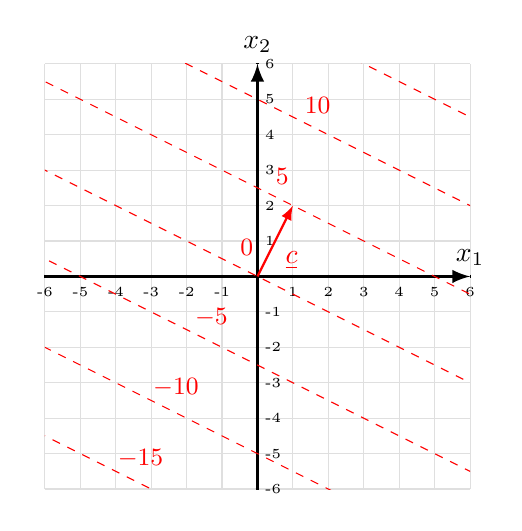
\begin{tikzpicture}[scale=0.45]

    \pgfmathtruncatemacro{\xa}{-6}
    \pgfmathtruncatemacro{\xb}{6}
    \pgfmathtruncatemacro{\ya}{-6}
    \pgfmathtruncatemacro{\yb}{6}
    \draw[gray!25, thin, step=1] (\xa,\ya) grid (\xb,\yb);
    \draw[very thick,-latex] (\xa,0) -- (\xb,0) node[above] {$x_1$};
    \draw[very thick,-latex] (0,\ya) -- (0,\yb) node[above] {$x_2$};

    \foreach \x in {\xa,...,\xb} \draw (\x,0.05) -- (\x,-0.05) node[below] {\ifthenelse{\x=0}{}{\tiny\x}};
    \foreach \y in {\ya,...,\yb} \draw (-0.05,\y) -- (0.05,\y) node[right=-0.5mm] {\ifthenelse{\y=0}{}{\tiny\y}};

    \pgfmathtruncatemacro{\vx}{1}
    \pgfmathtruncatemacro{\vy}{2}
    \draw[red,thick,-latex] (0,0) -- node[below right ,pos=0.5] {$\vecnot{c}$} (\vx,\vy);
	\begin{scope}
        \clip(\xa,\ya) rectangle (\xb,\yb);
		\foreach \i in {-4,...,4}
		    \draw[red,dashed] (\vx*\i+5*\vy,\vy*\i-5*\vx) -- node [red,pos=0.515,above=0.75mm] {\small\pgfmathparse{(\vx*\vx+\vy*\vy)*\i}\pgfmathprintnumber{\pgfmathresult}} (\vx*\i-5*\vy,\vy*\i+5*\vx);
	\end{scope}
		    
\end{tikzpicture}
\end{minipage}

\end{frame}

\begin{frame}{Constrained Linear Optimization}

\begin{minipage}{0.45\textwidth}
Now, consider the \textcolor{blue}{constrained} linear optimization problem:
\[ \min_{\vecnot{x} \in \mathcal{D}} \vecnot{c}^T \vecnot{x}. \]  

Figure shows $\color{green!40!black} \mathcal{D}$ with level sets of $\vecnot{c}^T \vecnot{x}$ for $n=2$ and $\color{red} \vecnot{c}=(1,2)$.

\vspace{3mm}

\visible<2->{ $\circ\,$~Optimal point $\color{blue} \vecnot{x}^*$ can be found using gradient descent from any initial feasible point.}

\vspace{2mm}

\visible<3->{ $\circ\,$~Negative gradient canceled by constraint normal to give feasible descent direction.}

\end{minipage}
\hfill
\begin{minipage}{0.50\textwidth}
\begin{tikzpicture}[scale=0.45]
    \pgfmathtruncatemacro{\xa}{-6}
    \pgfmathtruncatemacro{\xb}{6}
    \pgfmathtruncatemacro{\ya}{-6}
    \pgfmathtruncatemacro{\yb}{6}
    \draw[gray!25, thin, step=1] (\xa,\ya) grid (\xb,\yb);
    \draw[very thick,-latex] (\xa,0) -- (\xb,0) node[above] {$x_1$};
    \draw[very thick,->] (0,\ya) -- (0,\yb) node[above] {$x_2$};

    \foreach \x in {\xa,...,\xb} \draw (\x,0.05) -- (\x,-0.05) node[below] {\ifthenelse{\x=0}{}{\tiny\x}};
    \foreach \y in {\ya,...,\yb} \draw (-0.05,\y) -- (0.05,\y) node[right=-0.5mm] {\ifthenelse{\y=0}{}{\tiny\y}};

    \pgfmathtruncatemacro{\vx}{1}
    \pgfmathtruncatemacro{\vy}{2}
    \draw[red,thick,-latex] (0,0) -- node[below right ,pos=0.5] {$\vecnot{c}$} (\vx,\vy);
	\begin{scope}
        \clip(\xa,\ya) rectangle (\xb,\yb);
		\foreach \i in {-4,...,4}
		    \draw[red,dashed] (\vx*\i+5*\vy,\vy*\i-5*\vx) -- node [red,pos=0.515,above=0.75mm] {\pgfmathparse{(\vx*\vx+\vy*\vy)*\i}\pgfmathprintnumber{\pgfmathresult}} (\vx*\i-5*\vy,\vy*\i+5*\vx);
	\end{scope}

	\fill[green!50!black,opacity=0.25] (15/3,10/3) -- (1/3,-6/3) -- (13/3,-15/3) -- cycle;
	\draw (4.2,1.5) node[green!40!black] {$\mathcal{D}$};
	\only<2->{%
	  \draw (13/3,-15/3) node[circle,fill=blue,inner sep=1pt,node contents={}];
	  \draw (13/3,-15/3) node[below,blue] {$\vecnot{x}^*$};
	}
    \only<3->{%
      \draw[red,thick,-latex] (3,-4) -- (3-\vx/2,-4-\vy/2);
      \draw[green!40!black,thick,->] (3,-4) -- (3+3/5,-4+3/4);
      \draw[blue,thick,-latex] (3,-4) -- (3+2/3,-4-2/4);
    }
		
\end{tikzpicture}
\end{minipage}

\end{frame}


\begin{frame}{5.4: Constrained Non-Linear Optimization}

\iffalse
Lagrangian optimization is an indispensable tool in engineering and physics that allows one to solve constrained non-linear optimization problems.

\vspace{4mm}
\hrule
\vspace{4mm}
\fi

Consider a constrained non-linear optimization problem over $\mathcal{D} \subseteq \mathbb{R}^n$  in the following \textcolor{blue}{standard form}.
Let $f_i \colon \mathcal{D} \rightarrow \mathbb{R}$ and $h_j \colon \mathcal{D} \rightarrow \mathbb{R}$ be real functionals for $i=0,1,\ldots,m$ and $j=1,2,\ldots,p$.
Then, we write
\begin{align*}
\mathrm{minimize} \quad & f_0 (\vecnot{x}) \\
\mathrm{subject\,to} \quad & f_i (\vecnot{x}) \leq 0, \quad i=1,2,\ldots,m \\
& h_j (\vecnot{x}) = 0, \quad j=1,2,\ldots,p.
\end{align*}

\hrule

\begin{itemize}
\item<2-> the function $f_0$ is called the \textcolor{blue}{objective function}
\item<3-> the functions $f_1,\ldots,f_m$ define \textcolor{blue}{inequality constraints}
\item<4-> the functions $h_1,\ldots,h_p$ define \textcolor{blue}{equality constraints}
\item<5-> \textcolor{blue}{feasible} points in $\mathcal{F} \triangleq \{ \vecnot{x}\in \mathcal{D} \, | \,  f_i (\vecnot{x}) \leq 0, i\in [m], h_j (\vecnot{x}) = 0, j\in[p] \}$ satisfy all constraints and the problem is feasible if $\mathcal{F} \neq \emptyset$.
\item<6-> the \textcolor{blue}{optimal value} is $p^* \triangleq \inf \left\{ f_0 (\vecnot{x}) \, | \, \vecnot{x} \in \mathcal{F} \right\}$
\item<7-> problem called \textcolor{blue}{convex} if all $f_i$ convex and all $h_j$ affine: $h_j (\vecnot{x}) \!=\! \vecnot{a}_j^T \vecnot{x} \!-\! b_j \!\!\!$ 
\end{itemize}

\end{frame}

\begin{frame}{General Example}

\vspace{-2mm}

  \begin{center}
    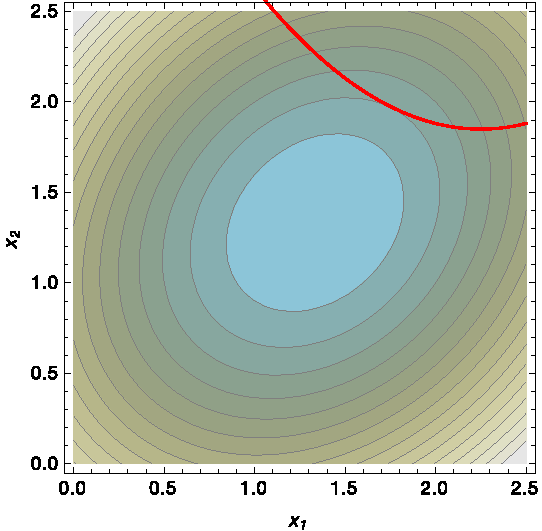
\includegraphics[width=65mm]{opt_fig}
  \end{center}

\vspace{-2mm}

Contour plot of $f_0 (x_1,x_2) = (x_1 - 1)^2 + (x_2 - 1)^2 - x_1 x_2 /2$ whose minimum occurs at $(4/3,4/3)$ (i.e., center of blue ellipse).  The red line shows the inequality constraint $f_1 (x_1,x_2)= 1.85 + (x_1 - 2.25)^2 / 2 - x_2 \leq 0$

\end{frame}

\begin{frame}{Linear Programs}

The optimization of a linear function with arbitrary affine equality and \\ inequality constraints is called a \textcolor{blue}{linear program (LP)}.

\vspace{3mm}

LPs have many equivalent forms because:
\begin{itemize}
\item $x_1 \!=\! 0$ is the same as $(x_1 \leq 0) \wedge (x_1\geq 0)$
\item $x_1 \leq 0$ is the same as $(x_1 + x_2 = 0) \wedge x_2 \geq 0$ for slack variable $x_2$
\item negation swaps: $\min \& \max$ for objective and $\geq \& \leq$ for constraints
\end{itemize}  

\begin{definition}
Any LP can be transformed into one of the standard $\min$ forms: \\[1mm]
\hrule \vspace{0mm}
\begin{minipage}{0.49\textwidth}
\vspace{-2mm}
\begin{align*}
\mathrm{minimize} \quad & \vecnot{c}^T \vecnot{x} \\
\mathrm{subject\,to} \quad & A \vecnot{x} = \vecnot{b} \\
& \vecnot{x} \succeq \vecnot{0}
\end{align*}
\end{minipage}
\vrule
\begin{minipage}{0.49\textwidth}
\vspace{-2mm}
\begin{align*}
\mathrm{minimize} \quad & \vecnot{c}^T \vecnot{x} \\
\mathrm{subject\,to} \quad & A \vecnot{x} \succeq \vecnot{b} \\
& \vecnot{x} \succeq \vecnot{0}
\end{align*}
\end{minipage}
\end{definition}

\end{frame}


\begin{frame}{Langrangian Formulation}

Used to transform from constrained to unconstrained optimization

\begin{definition}
For the standard optimization, the \textcolor{blue}{Lagrangian} $L \colon \mathcal{D} \times \mathbb{R}^m \times \mathbb{R}^p \rightarrow \mathbb{R}$ is \vspace{-2mm}
\[ L(\vecnot{x},\vecnot{\lambda},\vecnot{\nu}) = f_0(\vecnot{x}) + \sum_{i=1}^m \lambda_i f_i(\vecnot{x}) + \sum_{j=1}^p \nu_j h_j(\vecnot{x}), \vspace{-1.5mm} \]
where the \textcolor{blue}{Lagrange multipliers} $\lambda_i$ and $\nu_j$ define penalties associated with violating the $i$-th inequality and $j$-th equality constraints, respectively.
\end{definition}

\begin{theorem}[Karush-Kuhn-Tucker]<2->
Assume the functions $f_i$ and $h_j$ are continuously differentiable and let $A = \{ i\in [m] \, | \, f_i (\vecnot{x}^*)=0 \}$ be the set of active constraints at $\vecnot{x}^*$.
Then, $\vecnot{x}^*$ is locally optimal only if $\vecnot{\lambda}^* \geq 0$ and $\vecnot{\nu}^*$ exist such that \vspace{-1.5mm}
\begin{align*}
\nabla_\vecnot{x} L(\vecnot{x},\vecnot{\lambda},\vecnot{\nu}) = \nabla f_0 (\vecnot{x}^*) + \sum_{i\in A} \lambda_i^* \nabla f_i (\vecnot{x}^*) + \sum_{j=1}^p \nu_j^* \nabla h_j (\vecnot{x}^*) &= \vecnot{0} \vspace{-1mm}
\end{align*}
\end{theorem}

% Add example pic with vector additions

\end{frame}

\iffalse
\begin{frame}{Lagrangian Example}

For the pictured example, the Lagrangian is given by
\[ L(\vecnot{x},\lambda) = \underbrace{(x_1 \!-\! 1)^2 + (x_2 \!-\! 1)^2 - \frac{x_1 x_2}{2}}_{f_0(\vecnot{x})} + \lambda \Bigg( \underbrace{1.85 + \frac{(x_1 - 2.25)^2}{2} \!-\! x_2}_{f_1 (\vecnot{x})} \Bigg) \]

\centering
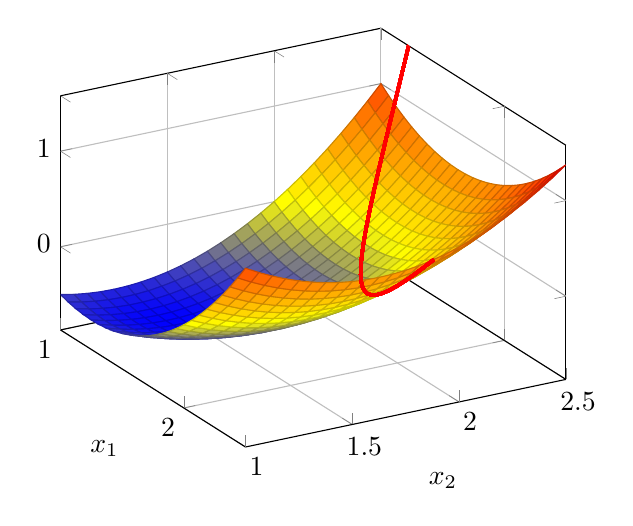
\begin{tikzpicture}
  \begin{axis}[width=80mm,view={60}{30},grid=major,ymin=1.0,ymax=2.5,xmin=1.0,xmax=2.5,xlabel=$x_1$,ylabel=$x_2$]
    \addplot3 [surf,domain=1:2.5] {(x-1)^2 + (y-1)^2 - x*y/2 + 0*(1.85+(x-2.25)^2/2-y)};
    %\addlegendentry{$\lambda=0$}
    
    %\addplot3 [surf,domain=1:2.5] {(x-1)^2 + (y-1)^2 - x*y/2 + 1*(1.85+(x-2.25)^2/2-y)};
    %\addlegendentry{$\lambda=1$}

    \addplot3 [variable=x,mesh,domain=1.0:2.5,red,very thick] ({x},{(1.85+((x-2.25)^2)/2)},{(x-1)^2 + ((1.85+((x-2.25)^2)/2)-1)^2 - x*(1.85+((x-2.25)^2)/2)/2});
    %\addlegendentry{$constraint$}
\end{axis}
\end{tikzpicture}
\end{frame}


\fi

\begin{frame}{Langrangian Duality}

\begin{definition}
The \textcolor{blue}{Lagrangian dual} function is defined to be \vspace{-1.5mm}
\[ g(\vecnot{\lambda},\vecnot{\nu}) \triangleq \inf_{\vecnot{x}\in \mathcal{D}} L(\vecnot{x},\vecnot{\lambda},\vecnot{\nu}) = \inf_{\vecnot{x}\in \mathcal{D}} \Bigg( f_0(\vecnot{x}) + \sum_{i=1}^m \lambda_i f_i(\vecnot{x}) + \sum_{j=1}^p \nu_j h_j(\vecnot{x}) \Bigg). \]
\end{definition}


%The pointwise infimum of linear functions is concave because
%\[ \inf_{\vecnot{x}\in \mathcal{D}} %L(\vecnot{x},\vecnot{\lambda},\vecnot{\nu})  \inf]

\begin{lemma}<2->
The Lagrangian dual function is concave and the dual problem \vspace{-2.5mm}
\begin{align*}
\mathrm{maximize} \quad & g(\vecnot{\lambda},\vecnot{\nu}) \\
\mathrm{subject\,to} \quad & \vecnot{\lambda} \geq 0 \vspace{-1mm}
\end{align*}
has a unique max value $d^* \leq p^*$.
This property is known as \textcolor{blue}{weak duality}.
\end{lemma}

\begin{definition}<3->
If $d^* = p^*$, then one says that \textcolor{blue}{strong duality} holds for the problem.
\end{definition}

\visible<3->{Proof of lemma on whiteboard}

\end{frame}

\begin{frame}{Weak Duality Proof}

Lagrangian dual is concave because pointwise infimum of affine functions:\vspace{-1mm}
\begin{align*}
g(\alpha\vecnot{\lambda}+&(1-\alpha)\vecnot{\lambda}',\alpha\vecnot{\nu}+(1-\alpha)\vecnot{\nu}') \\
&= \inf_{\vecnot{x}\in \mathcal{D}} L(\vecnot{x},\alpha\vecnot{\lambda}+(1-\alpha)\vecnot{\lambda}',\alpha\vecnot{\nu}+(1-\alpha) \vecnot{\nu}') \\
&= \inf_{\vecnot{x}\in \mathcal{D}} \big( \alpha L(\vecnot{x},\vecnot{\lambda},\vecnot{\nu}) + (1-\alpha) L(\vecnot{x},\vecnot{\lambda}',\vecnot{\nu}') \big) \\
&\geq \inf_{\vecnot{x}\in \mathcal{D}} \alpha L(\vecnot{x},\vecnot{\lambda},\vecnot{\nu}) + \inf_{\vecnot{x}'\in \mathcal{D}} (1-\alpha) L(\vecnot{x}',\vecnot{\lambda}',\vecnot{\nu}') \\
&= \alpha g(\vecnot{\lambda},\vecnot{\nu}) + (1-\alpha) g(\vecnot{\lambda}',\vecnot{\nu}'). \vspace{-1mm}
\end{align*}
Concavity implies unique maximum value $d^*$ upper bounded by \vspace{-2mm}
\begin{align*}
g(\vecnot{\lambda},\vecnot{\nu})
&= \inf_{\vecnot{x}\in \mathcal{D}} L(\vecnot{x},\vecnot{\lambda},\vecnot{\nu})
\stackrel{(a)}{\leq} \inf_{\vecnot{x}\in \mathcal{F}} L(\vecnot{x},\vecnot{\lambda},\vecnot{\nu}) \\
&\stackrel{(b)}{=} p^* + \sum_{i=1}^m \lambda_i f_i (\vecnot{x})
\stackrel{(c)}{\leq} p^*, \vspace{-3mm}
\end{align*}
where $(a)$ is implied by $\mathcal{F} \subseteq \mathcal{D}$, $(b)$ follows from $h_j(\vecnot{x}) = 0$ for $\vecnot{x}\in \mathcal{F}$, and $(c)$ holds by combining $f_i(\vecnot{x}) \leq 0$ for $\vecnot{x}\in \mathcal{F}$ and $\lambda_i \geq 0$.

\end{frame}

\backupbegin

%\begin{frame}
%\frametitle{Backup Slides}
%\begin{itemize}
%\item Slide numbers not included in denominator!
%\end{itemize}
%\end{frame}

%\begin{frame}[allowframebreaks]
%\frametitle{References}
%\bibliographystyle{alpha}
%\footnotesize
%\bibliography{IEEEabrv,WCLabrv,WCLbib,WCLnewbib}
%\end{frame}

\backupend

\end{document}
